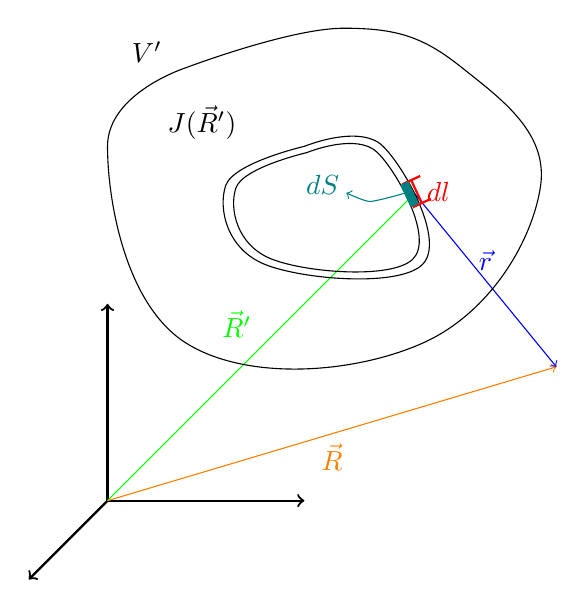
\begin{tikzpicture}
\draw [<->, thick](-1,1.5) -- (-1,-1) node (v1) {} -- (1.5,-1);
\draw [->, thick](v1.center) -- (-2,-2);
\draw [->, green] (v1.center) -- (2.9,2.9) node [midway,above left]{$\vec{R}'$};
\draw [->, orange](v1.center) -- (4.7,0.7) node [midway,below]{$\vec{R}$};
\draw [->, blue](2.9,2.9) -- (4.7,0.7) node [midway,above]{$\vec{r}$};
\draw  plot[smooth, tension=.7] coordinates {(1.5,3.5) (0.5,3) (1,2) (3,2) (2.5,3.5) (1.5,3.5)};
\draw [scale=0.9] plot[smooth, tension=.7] coordinates {(1.7,3.8) (0.7,3.3) (1.2,2.3) (3.2,2.3) (2.7,3.8) (1.7,3.8)};
\draw  plot[smooth, tension=.7] coordinates {(0,4.5) (-1,3.5) (0,1) (3,1) (4.5,3) (3.5,4.5) (2,5) (0,4.5)};

\draw [ thick, red,|-|] (2.8506,3.0831) -- (2.9976,2.7666) node[midway, right]{$dl$};
\draw [fill, teal, rotate=-65]  (-1.5715,3.8417) rectangle (-1.2715,3.7417);
\draw  [teal,->]plot[smooth, tension=.7] coordinates {(2.7662,2.9022) (2.414,2.8123) (2.2717,2.8123) (2.0319,2.9097)};
\node at (1.7321,3.0146) [teal]{$dS$};
\node at (0.2,3.8) {$J(\vec{R}')$};
\node at (-0.5,4.7) {$V'$};
\end{tikzpicture}